\chapter{Emisi\'on de ondas de radio de una EAS}
\label{ch:easRadio}

El objetivo de este cap\'itulo es ganar intuci\'on sobre la emisión de ondas de radio en lluvias atmosféricas extendidas.
Para ello, se abordar\'a el problema desde varios puntos de vista.
En primer lugar se revisar\'a el mecanismo mediante el cu\'al las EAS emiten una se\~nal de radio a nivel microsc\'opico, lo que permite calcular el campo de manera precisa. 
Luego se discutir\'an algunos mecanismos efectivos que se proponen para explicar el fen\'omeno, lo que permite estudiarlo desde un punto de vista m\'as intuitivo.
Se abordar\'a tanto la geometr\'ia de la emisi\'on como su polarizaci\'on y distribuci\'on del campo el\'ectrico a nivel del suelo.
Finalmente, se presenta un modelo simplificado desarrollado para, mediante razonamientos elementales, comprender las caracter\'isticas principales de la se\~nal emitida por eventos ES.

\section{Modelado de la emisi\'on}
\label{sc:gen_emision}

El modelado de la emisi\'on de radio de las lluvias atmosf\'ericas extendidas suele encararse de alguna de las siguientes maneras, mediante un enfoque microsc\'opico o utilizando un enfoque efectivo o macrosc\'opico

La mirada microsc\'opica consiste en obtener el campo el\'ectrico emitido por la lluvia como suma de las contribuciones de cada una de sus part\'iculas, mientras que el tratamiento efectivo propone representar la lluvia como una superposici\'on de cargas y corrientes equivalentes a partir de las que es posible obtener el campo electromagn\'etico total.
La ventaja m\'as importante que otorga la mirada microsc\'opica radica en la exactitud del c\'alculo realizado, que depende b\'asicamente de la capacidad de calcular correctamente la din\'amica de la generaci\'on de part\'iculas en una lluvia atmosf\'erica.
Por este motivo, y debido a la complejidad inherente del problema se lo aborda mediante t\'ecnicas de Monte Carlo, combinadas usualmente con un alto poder de c\'omputo.

Como contraparte, las ventajas de los modelos efectivos residen en la simplificaci\'on del problema, lo que disminuye la necesidad tiempo de CPU y al mismo tiempo facilita la interpretaci\'on intuitiva de los resultados. 
Sin embargo dicha reducci\'on deviene en un nuevo conjunto de par\'ametros, necesarios para lograr una representacion adecuada de las distribuciones de carga de la lluvia, y que necesitan de una calibraci\'on previa para entregar resultados confiables.

Si bien en esta Tesis se utiliza un modelo microsc\'opico para calcular la se\~nal sobre el detector, en las siguientes secciones se abordar\'an ambos enfoques, lo que facilitar\'a la interpretaci\'on de los resultados del cap\'itulo \ref{ch:simulacionRadio}.

\section{Modelado microsc\'opico}

El modelado microsc\'opico de una EAS se basa en calcular la emisi\'on de radio de cada part\'icula de la lluvia desde primeros principios (ecuaciones de Maxwell).
Luego, el campo total en un punto dado del espacio y a un tiempo determinado se obtiene sumando la contribuci\'on de cada una, es decir, aplicando el principio de superposici\'on del electromagnetismo y sin realizar hip\'otesis \emph{a priori} acerca del mecanismo dominante en la emisi\'on.
La idea central es representar la trayectoria de cada part\'icula cargada, en general curva, como una sucesi\'on de trazos rectos recorridos a velocidad constante, pero con diferente m\'odulo y direcci\'on en cada uno.
Entonces, resulta fundamental comprender el mecanismo mediante el cual cada part\'icula de la lluvia emite radiaci\'on.

\subsection{Emisi\'on de cada part\'icula de la lluvia}

En esta secci\'on se sigue los razonamientos desarrollados en \cite{alvarez:2013}, donde pueden encontrarse m\'as detalles sobre el tema.
El objetivo es encontrar las ecuaciones que describen el campo el\'ectrico generado por un electr\'on eyectado de un \'atomo de la atm\'osfera a tiempo $t=t_1$ que viaja a velocidad constante $\mathbf{v}$ hasta que es absorbido por otro \'atomo a tiempo $t_2$.
Si se desprecia el movimiento de los \'atomos, es posible modelar la corriente asociada a dicho proceso con la ecuaci\'on:
%
\begin{equation}
\mathbf{J}(\mathbf{x},t)=-e\mathbf{v}\delta^{(3)}(\mathbf{x}-\mathbf{x_o}-\mathbf{v}t)
\Theta(t-t_1)\Theta(t_2-t)
\label{eq:eCurrent}
\end{equation}
%
donde $e=|e|$ es la carga de un positr\'on, $\mathbf{x}$ describe la posici\'on respecto de la referencia $\mathbf{x_o}$.
La funci\'on $\Theta$ de Heaviside toma en cuenta el hecho de que el electr\'on se mueve libremente durante el intervalo de tiempo $(t_1,t_2)$.

En un medio diel\'ectrico de permitividad $\mathbf{\epsilon}$ y susceptibilidad magn\'etica $\mu$, la ecuaci\'on de Maxwell de dominio en frecuencias $\omega$ puede ser escrita como en la siguiente ecuaci\'on~\cite{jackson:1998}:
%
\begin{equation}
\nabla^2\mathbf{A}(\mathbf{x},\omega)+\mu\epsilon\omega^2\mathbf{A}(\mathbf{x},\omega)
-\nabla\left[
\nabla\cdot\mathbf{A}(\mathbf{x},\omega)-i\epsilon\mu\omega\phi(\mathbf{x},\omega)
\right]
=
-\mu\mathbf{J}(\mathbf{x},\omega)
\label{eq:maxA}
\end{equation}
%
donde $\phi(\mathbf{x},\omega)$ ($\mathbf{A}(\mathbf{x},\omega)$) es la transformada de Fourier del potencial escalar (vector) bajo la definici\'on $f(\omega)=\int_{-\infty}^\infty dt e^{i\omega t} f(t)$.
Eligiendo el gauge de Lorentz, la ecuaci\'on \ref{eq:maxA} queda:
%
\begin{equation}
\nabla^2\mathbf{A}+k^2\mathbf{A}
=
-\mu\mathbf{J}
\label{eq:maxA2}
\end{equation}
%
con $k=n\omega/c$, y $n$ el \'indice de refracci\'on del medio.
Es importante notar que el gauge de Lorentz en el dominio de frecuencias, que se escribe como en la ecuaci\'on \ref{eq:gaugeL}~\cite{jackson:1998}, implica que el potencial escalar se encuentra completamente determinado por la divergencia del potencial vector, por lo que s\'olo \'este \'ultimo es necesario para determinar completamente el campo en todo el espacio.
%
\begin{equation}
\nabla\cdot\mathbf{A}(\mathbf{x},\omega)=i\epsilon\mu\omega\phi(\mathbf{x},\omega)
\label{eq:gaugeL}
\end{equation}
%

La soluci\'on a la ecuaci\'on \ref{eq:maxA2} puede obtenerse integrando funciones de Green sobre los puntos fuente~\cite{jackson:1998}, como en la ecuaci\'on \ref{eq:greenF}.
%
\begin{equation}
\mathbf{A}(\mathbf{x},\omega)=\frac{\mu}{4\pi}\int d^3\mathbf{x}\textquotesingle
\frac{e^{ik|\mathbf{x}-\mathbf{x}\textquotesingle|}}{|\mathbf{x}-\mathbf{x}\textquotesingle|}
\mathbf{J}(\mathbf{x}\textquotesingle,\omega)
\label{eq:greenF}
\end{equation}
%
En \'esta, $\mathbf{x}$ representa la posici\'on del observador, mientras que $\mathbf{x}\textquotesingle$ la de la fuente.
Sin p\'erdida de generalidad puede suponerse que el electr\'on se desplaza en la direcci\'on $\hat z$. 
Si adem\'as en la ecuaci\'on \ref{eq:eCurrent} se hacen los siguientes reemplazos, $q=-e$; $Z(t)=\Theta(t-t_1)\Theta(t_2-t)$ y $P(\mathbf{x},t)=\delta^{(3)}(\mathbf{x}-vt\hat z-z_o\hat z)$, la ecuaci\'on \ref{eq:greenF} queda:
%
\begin{equation}
\mathbf{A}(\mathbf{x},\omega)=\frac{\mu}{4\pi}
qv\hat z
\int d^3\mathbf{x}\textquotesingle
dt\textquotesingle e^{i\omega t\textquotesingle}
\frac{e^{ik|\mathbf{x}-\mathbf{x}\textquotesingle|}}{|\mathbf{x}-\mathbf{x}\textquotesingle|}
Z(t\textquotesingle)P(\mathbf{x}\textquotesingle,t)
\label{eq:greenF2}
\end{equation}
%
Cabe destacar que como en el gauge de Lorentz, el potencial vector de una part\'icula que se desplaza en la direcci\'on $\hat{z}$ s\'olo tiene componente $z$ (ecuaci\'on \ref{eq:greenF2}), la ecuaci\'on \ref{eq:gaugeL} puede reescribirse:
%
\begin{equation}
	\renewcommand{\arraystretch}{2.5}
	\begin{array}{rcl}
	\nabla\cdot\mathbf{A}(\mathbf{x},\omega)&=&\dfrac{\partial A_z}{\partial z}\\
	&=&
	\dfrac{\mu}{4\pi}qv
	\displaystyle\int d^3\mathbf{x}\textquotesingle dt\textquotesingle
	Z(t\textquotesingle)P(\mathbf{x}\textquotesingle,t)\\
	& & \times
	e^{i\omega t\textquotesingle}
	\dfrac{e^{ik|\mathbf{x}-\mathbf{x}\textquotesingle|}}{|\mathbf{x}-\mathbf{x}\textquotesingle|}
	\left[ik-\dfrac{1}{|\mathbf{x}-\mathbf{x}\textquotesingle|}\right]
	\dfrac{(z-z\textquotesingle)}{|\mathbf{x}-\mathbf{x}\textquotesingle|}
	\end{array}
\label{eq:gaugeL2}
\end{equation}
%

Con todo esto, el campo el\'ectrico $\mathbf{E}(\mathbf{x},\omega)$ puede obtenerse a partir del potencial escalar y del potencial vector utilizando la ecuaci\'on \ref{eq:efieldFromA}~\cite{jackson:1998}.
%
\begin{equation}
	\mathbf{E}(\mathbf{x},\omega) = 
	-\nabla\phi(\mathbf{x},\omega) 
	+
	i\omega\mathbf{A}(\mathbf{x},\omega)
	\label{eq:efieldFromA}
\end{equation}
%

Dada la simetr\'ia cil\'indrica del problema, s\'olo es necesario calcular las componentes radial y en direcci\'on $z$, $E_\rho$ y $E_z$.
Entonces, teniendo en cuenta que el potencial vector s\'olo tiene componente $z$, estas componentes pueden escribirse como en las ecuaciones \ref{eq:Ero1} y \ref{eq:Ez1}.
%
\begin{equation}
E_\rho(\mathbf{x},\omega)=
-\partial_\rho\phi(\mathbf{x},\omega)
=
-\partial_\rho\frac{\nabla\cdot\mathbf{A}(\mathbf{x},\omega)}{i\mu\epsilon\omega}
\label{eq:Ero1}
\end{equation}
%
\begin{equation}
	\renewcommand{\arraystretch}{2.5}
	\begin{array}{rcl}
	E_z(\mathbf{x},\omega)& = & 
	-\partial_z\phi(\mathbf{x},\omega) + i\omega A_z(\mathbf{x},\omega)\\
	& = &
	-\partial_z\dfrac{\nabla\cdot\mathbf{A}(\mathbf{x},\omega)}{i\mu\epsilon\omega}
	+ i\omega A_z(\mathbf{x},\omega)
	\end{array}
\label{eq:Ez1}
\end{equation}
%
Finalmente, derivando \ref{eq:Ero1} y \ref{eq:Ez1} se obtienen las ecuaciones buscadas para el campo el\'ectrico:
%
\begin{equation}
	\renewcommand{\arraystretch}{2.5}
	\begin{array}{rcl}
	E_\rho(\mathbf{x},\omega)& = & 
	i\dfrac{qv}{\omega}\dfrac{1}{4\pi\epsilon}
	\displaystyle\int_{t_1}^{t_2}dt\textquotesingle
	e^{i\omega t\textquotesingle}\dfrac{e^{ikr}}{r^3}\rho\\
	&&\times
	(z-z_o-vt\textquotesingle)
	\left[
		b\left(
			b-\dfrac{1}{r}-1
		\right)
		+\dfrac{1}{r^2}
	\right]\\
	\end{array}
\label{eq:Ero2}
\end{equation}
%
\begin{equation}
	\renewcommand{\arraystretch}{2.5}
	\begin{array}{rcl}
	E_z(\mathbf{x},\omega)& = & 
	i\dfrac{qv}{\omega}\dfrac{1}{4\pi\epsilon}
	\displaystyle\int_{t_1}^{t_2}dt\textquotesingle
	e^{i\omega t\textquotesingle}\dfrac{e^{ikr}}{r^2}\\
	&&\times
	\left[
		b^2\dfrac{(z-z_o-vt\textquotesingle)^2}{r}
		+
		b^2\dfrac{(z-z_o-vt\textquotesingle)^2}{r^3}
		\right.
		\\
		&&
		\left.
		-b\left(
			\dfrac{(z-z_o-vt\textquotesingle)^2}{r^2}-1
		\right)\,
	\right]\\
	&&+
	i\omega\dfrac{\mu}{4\pi}qv
	\displaystyle\int_{t_1}^{t_2}dt\textquotesingle
	e^{i\omega t\textquotesingle}\dfrac{e^{ikr}}{r}
	\end{array}
\label{eq:Ez2}
\end{equation}
%
donde $r=r(t\textquotesingle)$ y $b=b(t\textquotesingle)$ seg\'un:
%
\begin{equation}
r(t\textquotesingle)
= |\mathbf{x}-\mathbf{x}\textquotesingle|
= \sqrt{\rho^2+(z-z_o-vt\textquotesingle)^2}
\end{equation}
%
y
%
\begin{equation}
b(t\textquotesingle) = ik-\dfrac{1}{r(t\textquotesingle)}
\end{equation}

Las ecuaciones \ref{eq:Ero2} y \ref{eq:Ez2} proveen la soluci\'on exacta para el campo el\'ectrico de una part\'icula que se desplaza a trav\'es de un trayecto finito rectilineo a velocidad constante, lo que a partir de aqu\'i denominaremos \emph{track}.

\subsection{Aproximaci\'on ZHS}
\label{sbsc:zhs_approx}

Usualmente, las ecuaciones \ref{eq:Ero2} y \ref{eq:Ez2} no tienen soluci\'on anal\'itica, por lo que se las debe integrar num\'ericamente.
Dado que en una lluvia atmosf\'erica de \cant{1}{EeV} pueden generarse del orden de $10^{10}$ part\'iculas, su resoluci\'on a nivel microsc\'opico se torna impracticable.
% Por este motivo los programas de simulaci\'on suelen utilizar aproximaciones mediante las cuales el c\'omputo del campo se obtiene a trav\'es de ecuaciones aritm\'eticas.
Para salvar este problema, Zas, Halzen y Stanev~\cite{1_halzen_zas_stanev_1991,2_zas_halzen_stanev_1992} propusieron un conjunto de aproximaciones, conocidas como \emph{aproximaciones ZHS}, que permiten salvar el problema, convirtiendo \ref{eq:Ero2} y \ref{eq:Ez2} en ecuaciones aritm\'eticas relativamente sencillas y adecuadas para su implementaci\'on en una simulaci\'on Monte Carlo. Las condiciones que se deben satisfacer son:
	%
	\begin{enumerate}
		\item La inversa de la distancia entre cualquier punto del track y el observador debe poder ser considerada una constante
		\begin{equation}
		\frac{1}{r(t)}\sim\frac{1}{R}
		\end{equation}
		\item La longitud del track es peque\~na en comparaci\'on con la distancia al observador. Esta condici\'on se traduce en $\eta\ll1$, con
		\begin{equation}
		\eta = \frac{k L^2}{R}\sin^2\theta
		\end{equation}
		donde $L\equiv v(t_1-t_2)$ es la longitud del track.
		\item El observador se encuentra en la zona de campo lejano
		\begin{equation}
		kR\gg1
		\end{equation}
	\end{enumerate}
	%
	Entonces, en estas circunstancias, el campo el\'ectrico $\vec{E}(t,\hat{u})$ en la posici\'on del observador puede calcularse mediante la ecuaci\'on \ref{eq:efield_0}.
	%
	\begin{equation}
	\renewcommand{\arraystretch}{2.5}
	\begin{array}{rl}
		\vec{E}(t,\hat{u})
		&=
		-\dfrac{\mu e}{4\pi Rc}
		\vec\beta_{\bot}\\
		& 
		\dfrac{\delta(t-\frac{nR}{c}-(1-n\beta\cos\theta)t_1)
			-\delta(t-\frac{nR}{c}-(1-n\beta\cos\theta)t_2)}{1-n\beta\cos\theta}
	\end{array}
	\label{eq:efield_0}
	\end{equation}
	%
	donde $\hat{u}$ es el versor que indica la direcci\'on entre la mitad del track y el observador, formando un \'angulo $\theta$ con el mismo. Mientras que $\vec\beta=\vec v/c$ y $\vec\beta_{\bot}=-[\hat{u}\times(\hat{u}\times\vec\beta)]$ es la proyecci\'on de $\vec\beta$ en la direcci\'on perpendicular a $\hat u$ sobre el plano que forman $\vec\beta$ y $\hat u$.
% 	y $t_{1,2}^{det}=t_{1,2}+nR/c-n\vec\beta \cdot \hat u (t_{1,2}-t_0)$ son los tiempos de detecci\'on del principio y final del track respectivamente, con $t_0=(t_1+t_2)/2$.
	Los detalles del c\'alculo para obtener \ref{eq:efield_0} a partir de \ref{eq:Ero2} y \ref{eq:Ez2} pueden encontrarse en \cite{alvarez:2013}.
	
	A partir de la ecuaci\'on \ref{eq:efield_0} puede calcularse el campo el\'ectrico emitido por cada part\'icula de la lluvia en ausencia de campos externos y para diferentes valores de $\theta$, lo que se esquematiza en la figura \ref{fig:zhs_pulse}.
	La caracter\'istica fundamental de la emisi\'on es que la radiaci\'on es producida en dos pulsos, uno al principio y otro al final de la trayectoria descripta, lo que resulta razonable si se tiene en cuenta que el camino se recorre a velocidad constante.
	Por otro lado, la separaci\'on temporal entre los pulsos, tal y como los ver\'ia el observador, viene dada por $\delta t = (1-n\beta\cos\theta)(t_2-t_1)$, que resulta de la resta entre los tiempos de emisi\'on y la diferencia de camino \'optico recorrido desde cada punto en que se emite.
	El \'angulo \cher{} $\theta_{cher}$\footnote{$\cos\theta_{cher}=\dfrac{1}{n\beta}$} resulta ser el que logra compensar estos efectos, logrando la mayor compresi\'on temporal entre los pulsos.
	De hecho, para $\theta\rightarrow\theta_{cher}$, $\delta t \rightarrow 0$ y el observador ve los dos pulsos al mismo tiempo.
	La diferencia de amplitud de cada pulso proviene de que formalmente en el caso limite $\theta\rightarrow\theta_{cher}$ el campo se obtiene como menos la derivada de la delta de Dirac, de lo que se obtiene un doble pulso que primero es antiparalelo a $\vec\beta$ y luego paralelo \cite{alvarez:2013}.
	%	
	\begin{figure}[ht!]
		\centering
		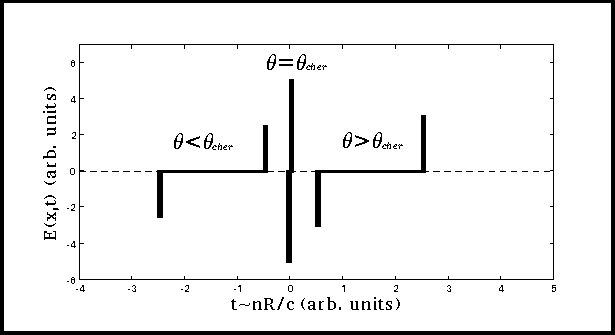
\includegraphics[width=0.75\textwidth]{fig/EASRadio/zhs_pulse}
		\caption{\label{fig:zhs_pulse} Tomado de \cite{alvarez:2013}. Representaci\'on esquematica del campo el\'ectrico emitido por un electr\'on que viaja con velocidad constante entre dos puntos para observadores posicionados a diferentes \'angulos respecto de su trayectoria. Ver detalles en el texto.}
	\end{figure}
	
	
\section{Modelado macrosc\'opico}
\label{sc:macroscopico}

Para explotar todo el potencial de un detector de antenas de radio es fundamental ganar intuici\'on sobre las caracter\'isticas de la se\~nal que se espera medir.
Para ello, resulta \'util abordar la emisi\'on de las lluvias atmosf\'ericas macrosc\'opicamente, reemplazando la din\'amica de la densidad de part\'iculas cargadas de la lluvia por cargas y corrientes efectivas cuyo campo el\'ectrico pueda ser calculado de manera sencilla mediante las ecuaciones de Maxwell.
En esta direcci\'on, se ha determinado experimentalmente~\cite{ardouin2005radio,huege2012lopes,horandel2009lofar,schroder2013tunka,kelley2011aera,} que existen dos efectos que dominan la emisi\'on de radiaci\'on en EAS: la deflexi\'on de las part\'iculas cargadas debido al campo geomagn\'etico y el desarrollo de un exceso de carga generado, por ejemplo, a medida que el frente de la lluvia incorpora electrones de los \'atomos atmosf\'ericos~\cite{scholten:2008}.
Estos, se denominan efecto geomagn\'etico y efecto Askaryan, respectivamente y se desarrollan en las secciones \ref{sbsc:geom_emision} y \ref{sbsc:ask_emision}.

Por otro lado, dado que las part\'iculas cargadas que se incorporan a la EAS se desplazan a una velocidad mayor a la de la luz en la atm\'osfera\footnote{El \'indice de refracci\'on de la atm\'osfera a nivel del suelo es $n\sim1.0003>1$} se produce efecto \cher{}.
Esto permite hacer predicciones sobre el comportamiento de la amplitud de la huella de radio a nivel del suelo y en particular, es la base del modelo simplificado que se presenta en la secci\'on \ref{sc:toymodel} para emisi\'on en eventos ES. 
La emisi\'on \cher{} de las EAS se desarrolla en la secci\'on \ref{sbsc:cher_emision}.

Finalmente, en la secci\'on \ref{sbsc:other_emision} se hace un recuento de otros efectos de segundo orden en la emisi\'on de radio de una cascada atmosf\'erica.

\subsection{Efecto geomagn\'etico}
\label{sbsc:geom_emision}
	
	El denominado efecto geomagn\'etico engloba el campo generado por la corriente efectiva que generan las part\'iculas cargadas de la lluvia al deflectarse debido al campo magn\'etico terrestre.
	Durante la evoluci\'on de la EAS, debido a la fuerza de Lorentz los \el{+} y \el{-} se desv\'ian en direcciones opuestas, lo que produce una corriente el\'ectrica, tal como se esquematiza en el panel izquierdo de la figura \ref{fig:geom_sketch}.
	Si bien la intensidad de esta corriente depende del tiempo de una manera complicada\footnote{La intensidad de la corriente depende, entre otros factores, de la distribuci\'on longitudinal de part\'iculas de la lluvia.}, su direcci\'on viene dada b\'asicamente por $\vec\beta\times \vec B$, donde $\vec \beta$ es paralelo al eje de la lluvia y $\vec B$ es el campo magn\'etico. 
	De esto resulta que es pr\'acticamente perpendicular tanto al eje de la lluvia como al campo magn\'etico terrestre \cite{kahn:1966}.
	En consecuencia el campo el\'ectrico generado posee una polarizaci\'on casi uniforme sobre la superficie de la tierra, lo que se observa en el panel derecho de la figura \ref{fig:geom_sketch}.
	Por otra parte, debido a que la magnitud de la corriente efectiva depende fuertemente de la velocidad de drift de los \el{+} y \el{-}, que a su vez depende directamente de la densidad de la atm\'osfera, este es el mecanismo de generaci\'on predominante cuando la lluvia se inicia a profundidades peque\~nas~\cite{requiered} (siempre y cuando $\vec\beta$ no sea paralelo a $\vec B$).
	%
	\begin{figure}[ht!]
		\centering
		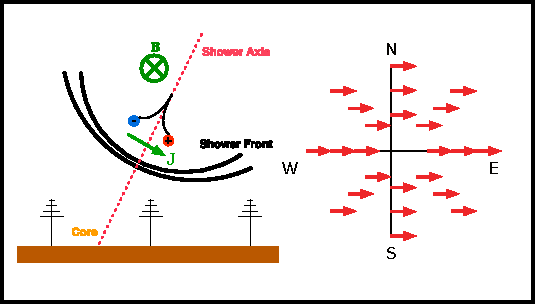
\includegraphics[width=0.75\textwidth]{fig/EASRadio/geom_sketch}
		\caption{\label{fig:geom_sketch} Izquierda: representaci\'on del efecto geomagn\'etico. Derecha: polarizaci\'on del campo el\'ectrico generado por el efecto geomagn\'etico a nivel del suelo en una cascada vertical. La variaci\'on en amplitud no se encuentra representada.}
	\end{figure}
	
\subsection{Efecto Askaryan}
\label{sbsc:ask_emision}
	
	El segundo mecanismo de emisión en importancia fue propuesto por Askaryan en 1962 \cite{askaryan1962} y se basa en que tanto el efecto Compton como la generaci\'on de rayos delta provocan un exceso de carga negativa durante el desarrollo de la lluvia.
	Este exceso es a su vez favorecido por la aniquilaci\'on de los positrones del frente de part\'iculas con los electrones de los \'atomos atmosf\'ericos. 
	Como consecuencia, aparece una carga efectiva que se mueve con la lluvia y que sigue en magnitud su desarrollo longituinal, o sea que primero crece, alcanza su m\'aximo y luego decrece.
	El panel izquierdo de la figura \ref{fig:ask_sketch} muestra un esquema del efecto Askaryan.
	
	Esta carga efectiva genera un campo proporcional a $-\left[\hat u \times \hat u \times \vec\beta\right]$\cite{cite:zhsPhysRevD}, donde $\hat u$ es la direcci\'on entre la carga que se desplaza y el observador\cite{jackson:1998}.
	Por ende, el campo eléctrico producido se encuentra polarizado en dirección aproximadamente radial en el plano de la cascada.
	A nivel del suelo y para una lluvia vertical, la componente Askaryan es tal como se esquematiza en el panel derecho de la figura \ref{fig:ask_sketch}.
	%
	\begin{figure}[ht!]
		\centering
		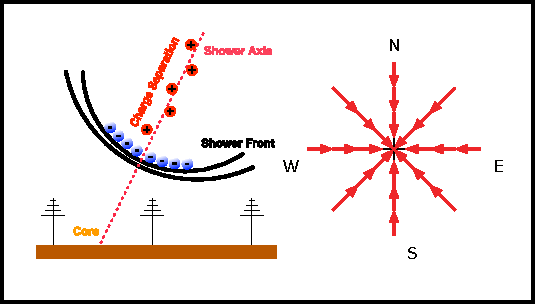
\includegraphics[width=0.75\textwidth]{fig/EASRadio/ask_sketch}
		\caption{\label{fig:ask_sketch} Izquierda: representaci\'on del efecto Askaryan.
		Derecha: polarización del campo eléctrico generado por el efecto Askaryan a nivel del suelo para una lluvia vertical. La variaci\'on en amplitud no se encuentra representada.}
	\end{figure}
	
	Es importante notar en este punto que tanto la polarizaci\'on del campo generado por el efecto geomagn\'etico como por el Askaryan es aproximadamente perpendicular al eje de la lluvia.
	Esta caracter\'istica resultar\'a de suma importancia a la hora de reconstruir la lluvia.
	
\subsection{Efecto \cher{}}
\label{sbsc:cher_emision}
	
	Las cargas y corrientes inducidas durante el desarrollo de una lluvia atmosf\'erica se desplazan a una velocidad mayor a la de la luz en la atm\'osfera, lo que provoca efecto \cher{}.
	Dado que su \'indice de refracci\'on difiere en algunas diezmil\'esimas del del vac\'io, el \'angulo \cher{} de la emisi\'on es peque\~no, como se observa en la ecuación \ref{eq:chAngle}, que muestra una estimación de su valor,
	%
	\begin{equation}
	\cos\theta_{cher} = \frac{1}{n} \sim \frac{1}{1.0003}
	\,\, \Rightarrow \,\,
	\theta_{cher} \sim 1.4^\circ
	\label{eq:chAngle}
	\end{equation}
	De aqu\'i se desprende que la emisi\'on \cher{} de radio de las EAS es esencialmente \emph{forward}, en la direcci\'on de la lluvia.
	Adem\'as, el hecho de que la corriente geomagn\'etica o el exceso de carga del efecto Askaryan se propagan a velocidad $>c/n$ en la atm\'osfera produce la aparici\'on de efectos de tipo \cher{} a nivel macrosc\'opico, a saber:
% 	Existen dos resultados interesantes que se desprenden de que la emisi\'on de la lluvia presente efecto \cher{}:
	\begin{enumerate}
	 \item La aparici\'on de lo que se denomina anillo \cher{}.
	 \item El aumento de la coherencia en frecuencia sobre dicho anillo.
	\end{enumerate}

	
	\subsubsection{Amplitud de la se\~nal a nivel del suelo: anillo \cher{}}
	\label{sbsc:cher_emision2}
	Al combinar la din\'amica de la lluvia con el efecto \cher{}, aparece una regi\'on a nivel del suelo sobre la que se espera un incremento en la se\~nal, denominado \emph{anillo \cher{}}.
	Para comprender la situaci\'on resulta \'util primero evaluar las diferencias entre la emisi\'on de una fuente de radiaci\'on que se desplaza a una velocidad menor y otra mayor a la de propagaci\'on de las ondas en el medio, lo que se esquematiza en la figura \ref{fig:cher_emision_1}.
	%
	\begin{figure}[ht!]
		\centering
		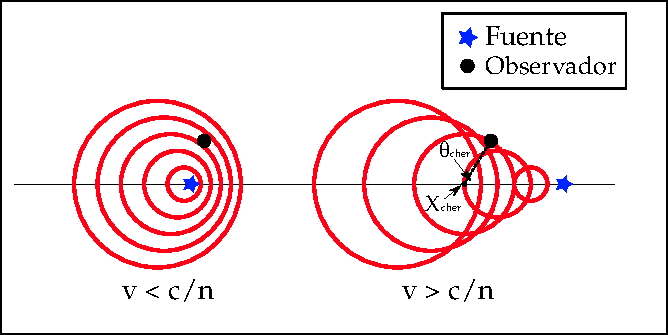
\includegraphics[width=0.85\textwidth]{fig/EASRadio/cherEmmision}
		\caption{\label{fig:cher_emision_1} Izquierda (derecha) esquema de los frentes de onda generados por un emisor que se desplaza a una velocidad menor (mayor) que la de propagaci\'on en el medio. Se observa como la recepci\'on del observador conserva el orden temporal en el que fueron emitidos los frentes en el caso $v<c/n$. Por otro lado, cuando el emisor se desplaza con velocidad $v>c/n$ el primer frente en alcanzar al observador es el que se emite cuando la direcci\'on de propagaci\'on del emisor forma el \'angulo \cher{} con la recta que lo une a la posici\'on del observador.}
	\end{figure}
	%
	Con este ejemplo, se busca destacar que cuando la velocidad del emisor es menor a la de propagaci\'on de las ondas en el medio, $v<c/n$, los frentes de onda alcanzan al observador en el mismo \'orden que fueron emitidos, mientras que cuando la velocidad de movimiento del emisor es tal que $v>c/n$ esto no siempre sucede.
	En el segundo caso, el primer frente de onda que interact\'ua con el observador es el que fue emitido en $x_{cher}$, determinado por el instante en el que la direcci\'on de movimiento de la fuente y la recta que une al emisor con el observador forman el \'angulo \cher{} (panel derecho de la figura \ref{fig:cher_emision_1}).
	Luego de recibir el primer frente, el observador ser\'a alcanzado simult\'aneamente por los emitidos antes y despu\'es de pasar por $x_{cher}$.
	Como resultado, si bien se pierde el orden temporal entre la se\~nal recibida y el proceso de emisi\'on, es posible asociar el inicio de la se\~nal en un dado observador con una posici\'on dada de la fuente.
% 	Adem\'as, la interferencia constructiva entre los frentes simult\'aneos que arriban luego del primer frente 
	
	Este \'ultimo resultado es muy \'util cuando adem\'as de este efecto se tiene en cuenta que la intensidad de la se\~nal recibida crece con la cantidad de part\'iculas presentes en la lluvia.
	As\'i, es posible predecir el comportamiento que tendr\'a la amplitud m\'axima de la se\~nal a nivel del suelo, lo que se esquematiza en la figura~\ref{fig:cher_emision_2}.
	%
	\begin{figure}[ht!]
		\centering
		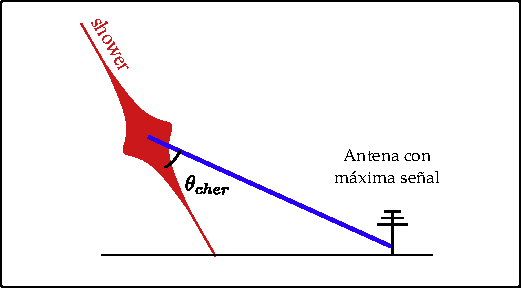
\includegraphics[width=0.85\textwidth]{fig/EASRadio/cono}
		\caption{\label{fig:cher_emision_2} Evoluci\'on de la se\~nal de radio emitida por una lluvia, a nivel del suelo. Se observa el mapeo que se produce entre los observadores y las diferentes etapas de la lluvia. Se destaca como la antena que observa la posici\'on en la que se produce el m\'aximo de part\'iculas registrar\'a mayor amplitud de se\~nal.}
	\end{figure}
	%
	En \'esta se muestra por un lado, como se produce el mapeo entre las diferentes etapas de evoluci\'on de la lluvia y los observadores a nivel del suelo, y por otro como el m\'aximo de amplitud de la se\~nal se espera en la antena que \emph{mira} la posici\'on de la lluvia en la que se produjo la mayor densidad de part\'iculas.
	Esto ha sido corroborado mediante simulaciones por ejemplo en \cite{zhairezAir}.
	
	Si se considera ahora que el detector es una red bidimensional de antenas, el m\'aximo de amplitud se hallar\'a en la intersecci\'on entre el plano del suelo y el cono \cher{} que procede de punto en el que la lluvia alcanza su m\'aximo. Esta regi\'on de m\'axima se\~nal se denomina anillo \cher{}, y se representa en la figura \ref{fig:cono}.
	%
	\begin{figure}[ht!]
		\centering
		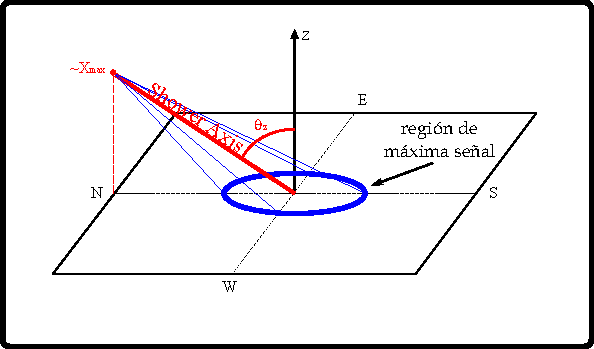
\includegraphics[width=0.7\textwidth]{fig/EASRadio/chConeSch}
		\caption{\label{fig:cono} La región de máxima señal a nivel del suelo se encuentra en la intersección entre el cono \cher{} que se proyecta desde el máximo de la lluvia y el suelo. Esta regi\'on se denomina anillo \cher{}.}
	\end{figure}
	%
	
	Si bien el \'indice de refracci\'on disminuye con la altitud~\cite{zhairezAir}, lo que provoca que el \'angulo \cher{} se haga m\'as pr\'oximo a $0^\circ$, los efectos aqu\'i descriptos no cambian.  
	
	\subsubsection{Coherencia de la se\~nal seg\'un la posici\'on del observador}
	
	La segunda consecuencia importante de que la emisi\'on de las lluvias atmosf\'ericas presenten efecto \cher{} se manifiesta en la frecuencia hasta la que se mantiene la coherencia de la se\~nal en diferentes regiones del suelo, alcanzando su m\'aximo sobre el anillo \cher{}.
	
	Este fen\'omeno es tambi\'en conocido como compresi\'on temporal y puede comprenderse si se analiza la siguiente situaci\'on simplificada.
	Se considera una antena ubicada a un \'angulo $\theta$ del eje de la lluvia, unidimensional y en un dado momento de su evoluci\'on, determinado por la posici\'on de su frente $l$ y por la densidad de part\'iculas $\rho(l)=dN(l)/dl$ (ver figura \ref{fig:coherencia_1}).
	En ese dado instante, si se supone que hay un exceso de nuevas part\'iculas generadas entre $l$ y $l+dl$, s\'olo para fijar ideas puede considerarse que se emitir\'an $dN_e$ pulsos  (una fracci\'on de las $dN$) que alcanzar\'an la antena entre los tiempos $0$ y $dt'=(1-n\cos\theta)\,dt$~\footnote{Esta expresi\'on se obtiene a partir de considerar los tiempos de llegada a la antena de dos pulsos emitidos desde $l$ y $l+dl$ a tiempos $0$ y $dt$ respectivamente, de tener en cuenta su propagaci\'on en el medio de indice de refracci\'on $n$ y haciendo la suposici\'on de que la distancia a la antena es mucho mayor que $dl$.}, donde $dt=dl/c$ y $c$ es la velocidad de propagaci\'on del frente de la lluvia.
	Esta situaci\'on se esquematiza en la figura \ref{fig:coherencia_1}.
	%
	\begin{figure}[ht!]
		\centering
		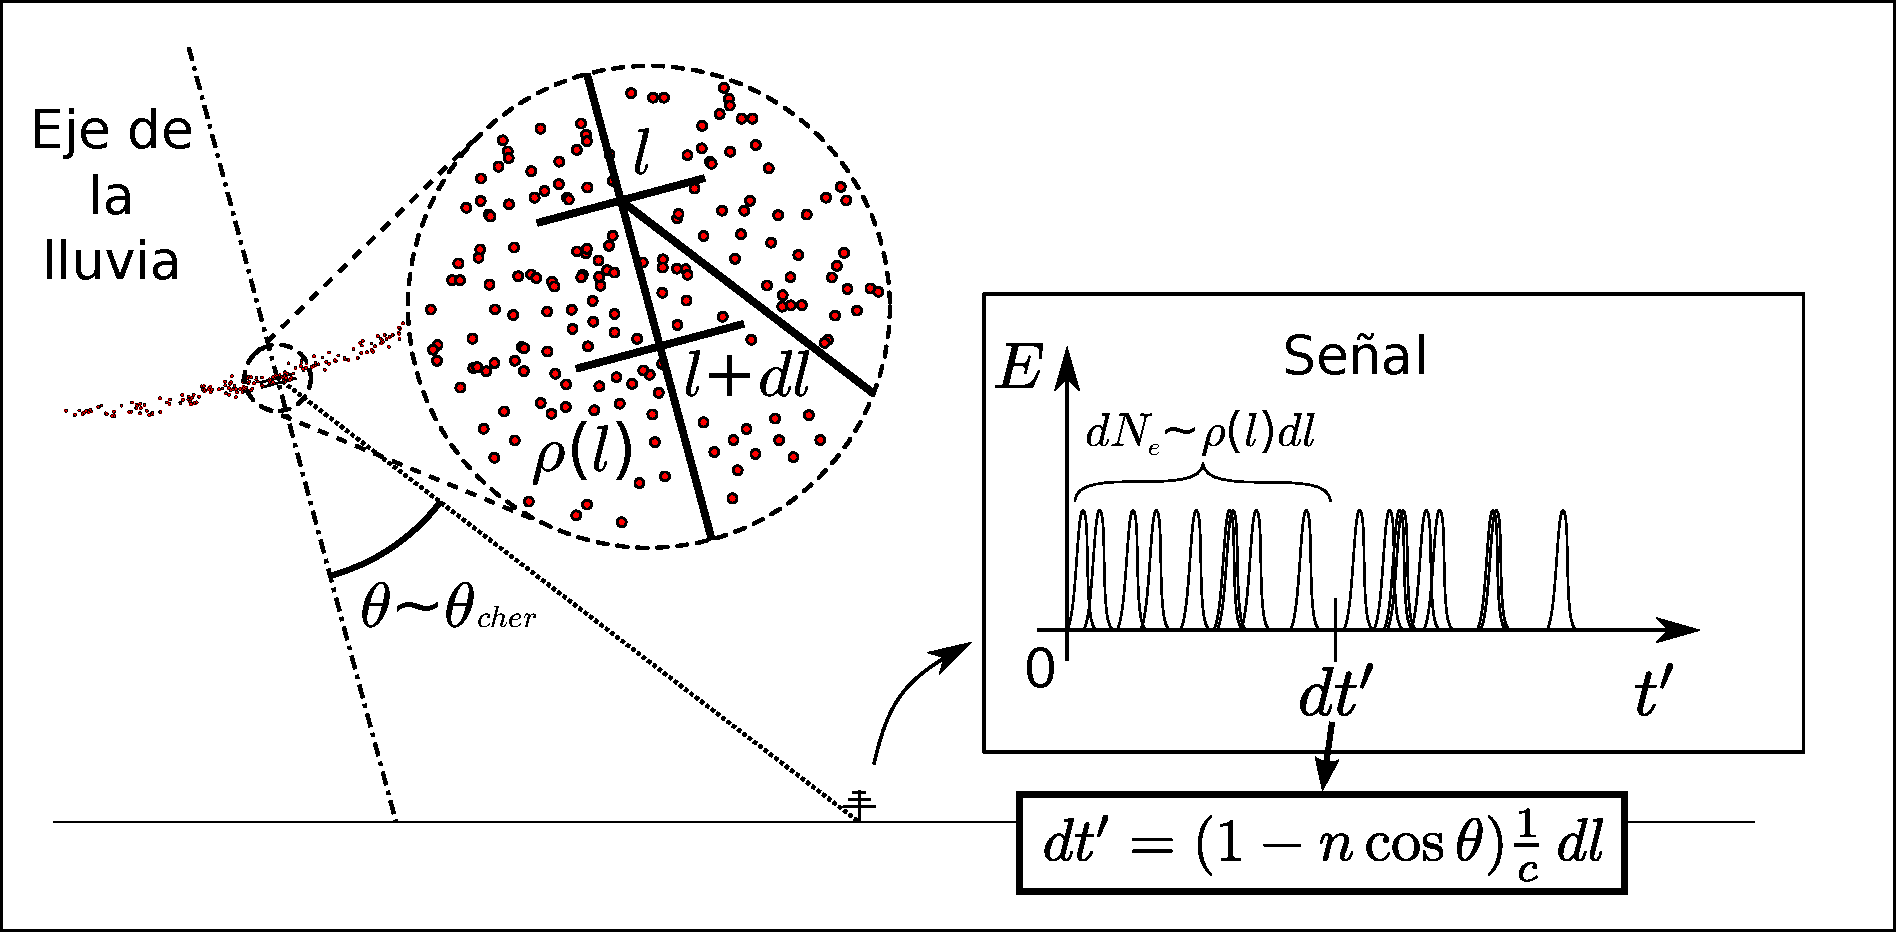
\includegraphics[width=0.9\textwidth]{fig/EASRadio/coherencia_2}
		\caption{\label{fig:coherencia_1} Esquema de la situaci\'on simplificada. En $dt'=(1-n\cos\theta)dt$ la antena ubicada aproximadamente en el \'angulo \cher{} recibir\'a $dN_e$ pulsos provenientes de las part\'iculas ubicadas entre $l$ y $l+dl$. Resulta razonable suponer que $dN_e$ es proporcional a la cantidad de part\'iculas presentes en la zona de emisi\'on $\rho(l)dl$.}
	\end{figure}
	%
	
	Si adem\'as se supone que la densidad lineal de emisores $\rho_e(l) = dN_e(l)/dl$ es proporcional a la densidad de part\'iculas presentes en ese lugar de la lluvia, $\rho(l)$, la ecuaci\'on para $dt'$ puede reescribirse como:
	%
	\begin{equation}
	 dt' = \frac{dl}{c}(1-n\cos\theta) = \frac{dN_e}{\rho_e(l) c}(1-n\cos\theta)\propto \frac{dN_e}{\rho(l) c}(1-n\cos\theta)
	 \label{eq:dt1}
	\end{equation}
	%
% 	o lo que resulta equivalente, dado que la se\~nal $dS$ integrada en el intervalo $dt'$ es proporcional a $dN_e$:
% 	%
% 	\begin{equation}
% 	 dS\propto\frac{\rho(l)c\ dt'}{(1-n\cos\theta)}
% 	 \label{eq:dS1}
% 	\end{equation}
	%
	
% 	Entonces, hasta aqu\'i vale la pena resaltar dos resultados interesantes:
% 	\begin{enumerate}
% 	 \item La \emph{compresi\'on temporal} con la que llegan los pulsos emitidos en $dl$ al observador se maximiza si $\theta\rightarrow\theta_{cher}=\frac{1}{n}$, dado que $dt'\rightarrow0$.
% 	 \item La amplitud acumulada en $dt'$ se vuelve m\'axima si 
% 	\end{enumerate}

	A $\theta$ fijo y considerando s\'olo los pulsos que provienen de $dl$, si se supone que para que la se\~nal pueda ser medida es necesario recibir al menos $dN_e^{min}$ pulsos dentro de cada intervalo $dt'$~\footnote{Esto puede lograrse agrandando $dl$ lo suficiente, hasta $dl_{min}$.}, queda definido un intervalo de tiempo m\'inimo $dt'_{min}$ sobre el que habr\'ia que integrar las se\~nales individuales para poder obtener alg\'un registro. A partir de \ref{eq:dt1} se tiene entonces:
	%
	\begin{equation}
	 dt'_{min} \propto \frac{dN_e^{min}}{\rho(l) c}(1-n\cos\theta)
	\end{equation}
	%
	Bajo estas suposiciones la componente de m\'axima frecuencia de la se\~nal $f_{max}$  ser\'a aproximadamente:
	%
	\begin{equation}
	 f_{max}\equiv \frac{1}{dt'_{min}} \propto \frac{\rho(l) c}{dN_{min}(1-n\cos\theta)}
	\end{equation}
	%
	donde el resultado importante es que $f_{max}\sim\rho(l)$. 
	Esto implica que las antenas que observan\footnote{En el sentido definido en la secci\'on \ref{sbsc:cher_emision2}.} el m\'aximo de part\'iculas de la lluvia, no s\'olo registrar\'an una se\~nal de mayor amplitud, sino que adem\'as \'esta mostrar\'a coherencia hasta frecuencias m\'as altas.
	
% 	En una situacion m\'as realista los c\'alculos se vuelven m\'as complicados debido a que las distintas regiones de la lluvia se ven con distintos valores de $\theta$ y a distintas distancias, la lluvia no es unidimensional o 
% 	Sin embargo
% que ve el maximo de la lluvia en el angulo Cherenkov detecta la señal de mayor 
% amplitud y de coherencia hasta frecuencias mas altas tal y como se ve en las 
% simulaciones y en la figura de  las "catedrales" que ya muestras al final de 2.3.3
	En una situacion m\'as realista los c\'alculos se vuelven complicados\footnote{Por ejemplo debido a que se ha despreciado el impacto que podr\'ia generar la cancelaci\'on con los pulsos generados por las part\'iculas absorbidas por \'atomos de la atm\'osfera, el caracter estoc\'astico subyacente, que la lluvia no es unidimensional, o que distintas regiones de la lluvia se ven con distintos valores de $\theta$ y a distintas distancias.}, sin embargo, este efecto se observa en simulaciones detalladas.
	Por ejemplo, la figura \ref{fig:chConeSig} muestra la amplitud de la señal en el suelo a diferentes frecuencias como función de la coordenada Este-Oeste de una lluvia, obtenida a partir de simulaciones.
	\begin{figure}[ht!]
	\centering
		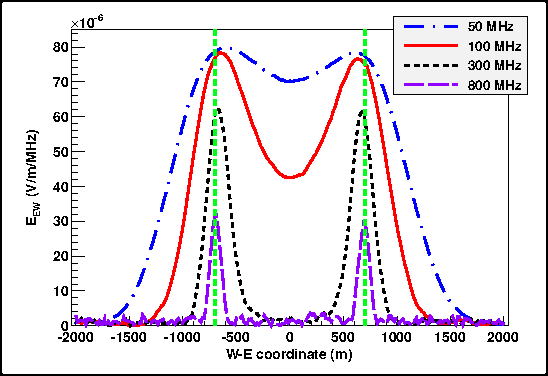
\includegraphics[width=0.7\textwidth]{fig/EASRadio/chConeSig}
		\caption{\label{fig:chConeSig} Amplitud del espectro de se\~nal en el suelo como funci\'on de la coordenada Este-Oeste de a lluvia obtenido a partir de simulaciones. En l\'inea punteada verde se grafica la posici\'on de impacto del cono \cher{}}
	\end{figure}
	En l\'ineas verdes, y en coincidencia con los máximos para todas las frecuencias se resalta el anillo \cher{} en esa coordenada.
	Se observa como a medida que la frecuencia filtrada aumenta la coherencia de la se\~nal se mantiene sólo en las cercan\'ias de dicho anillo.
	Este comportamiento en la se\~nal se conoce dentro del ambiente como las \emph{catedrales} del evento\footnote{Este nombre procede de que la forma de la se\~nal rememora las torres de una catedral.}.
	
\subsection{Otros efectos}
\label{sbsc:other_emision}
	
	Adem\'as de los mecanismos geomagn\'etico, Askaryan y \cher{} existen otros que si bien afectan la emisi\'on de radio de las cascadas atmosf\'ericas, lo hacen en menor medida. 
	A continuaci\'on se realiza un recuento de los mismos.
	
	\subsubsection{Efecto geosincrotr\'on}
	Los electrones y positrones de la lluvia, adem\'as de ser separados, son acelerados en su interacci\'on con el campo geomagn\'etico, que curva sus trayectorias.
	En este proceso se emite radiaci\'on de sincrotr\'on que, segun estudios te\'oricos recientes~\cite{geosintrotron}, representan una contribuci\'on menor en la emisi\'on total de la lluvia.
	
	\subsubsection{Campos electricos atmosf\'ericos}
	Los campos el\'ectricos atmosf\'ericos tambi\'en son capaces de acelerar las part\'iculas cargadas de las EAS, generando una contribuci\'on a veces considerable a la emisi\'on total de la lluvia. 
	Por ejemplo, durante per\'iodos de tormentas el\'ectricas el campo en la atm\'osfera puede alcanzar niveles de \cant{E_{atm}\sim10000}{V/m}, por lo que este fen\'omeno puede ser incluso mayor que el del efecto geomagn\'etico~\cite{atmosphericField}.
	Sin embargo, dado que usualmente los experimentos descartan los datos registrados en per\'iodos de tormenta y adem\'as, en condiciones normales los valores del campo atmosf\'erico rondan \cant{E_{atm}\sim100}{V/m}, su efecto suele despreciarse.
	
	
	\subsubsection{Bremsstrahlung molecular}
	
	La emisi\'on de radio debido a efecto de bremsstrahlung molecular generado por cascadas de part\'iculas fue medido recientemente en experimentos de aceleradores~\cite{bremsstrahlungMolec} y su coherencia fue medida a frecuencias del orden de los $\rm GHz$.
	Sin embargo, otros experimentos en aceleradores no han confirmado estas mediciones~\cite{AMY}.
	De todas formas varios experimentos comenzaron el desarrollo de t\'ecnicas especializadas para medir lluvias atmosf\'ericas extendidas en estas frecuencias, pero todav\'ia sin \'exito~\cite{cite:midas}\footnote{Salvo en los casos como en \cite{cite:CHROME} en los que se recibe una se\~nal proveniente de una lluvia con direcci\'on hacia el observador, lo que indica que en realidad y muy probablemente han medido la contribuci\'on geomagn\'etica de alta frecuencia (\cant{\sim}{GHz}) de la misma.}.
	Actualmente no es claro si el bremsstrahlung molecular constribuye de manera significativa a la emisi\'on en el \'orden de los $\rm MHz$.
	
\section{Emisi\'on de radio en eventos ES}
\label{sc:toymodel}
	
	Esta secci\'on profundiza en el estudio de la emisi\'on de radio en lluvias atmosf\'ericas extendidas a eventos ES. 
	La principal diferencia entre las lluvias verticales y los eventos ES radica en su geometr\'ia.
	Debido a que, como se expuso en la secci\'on \ref{sbsc:cher_emision}, la geometr\'ia juega un papel fundamental en la emisi\'on de radio de las EAS fuertemente influenciada por efectos del tipo \cher{}, es esencial estudiar los cambios que implica que los eventos sean ascendentes.
	
	\subsection{Anillo \cher{} en eventos ES}
	\label{sbsc:conoEs}
	
	La proyección sobre el suelo del cono \cher{} en eventos ES no es una elipse (o anillo) sino una hipérbola, como se grafica de manera esquem\'atica en la figura \ref{fig:chConeES}.
	\begin{figure}[ht!]
	\centering
		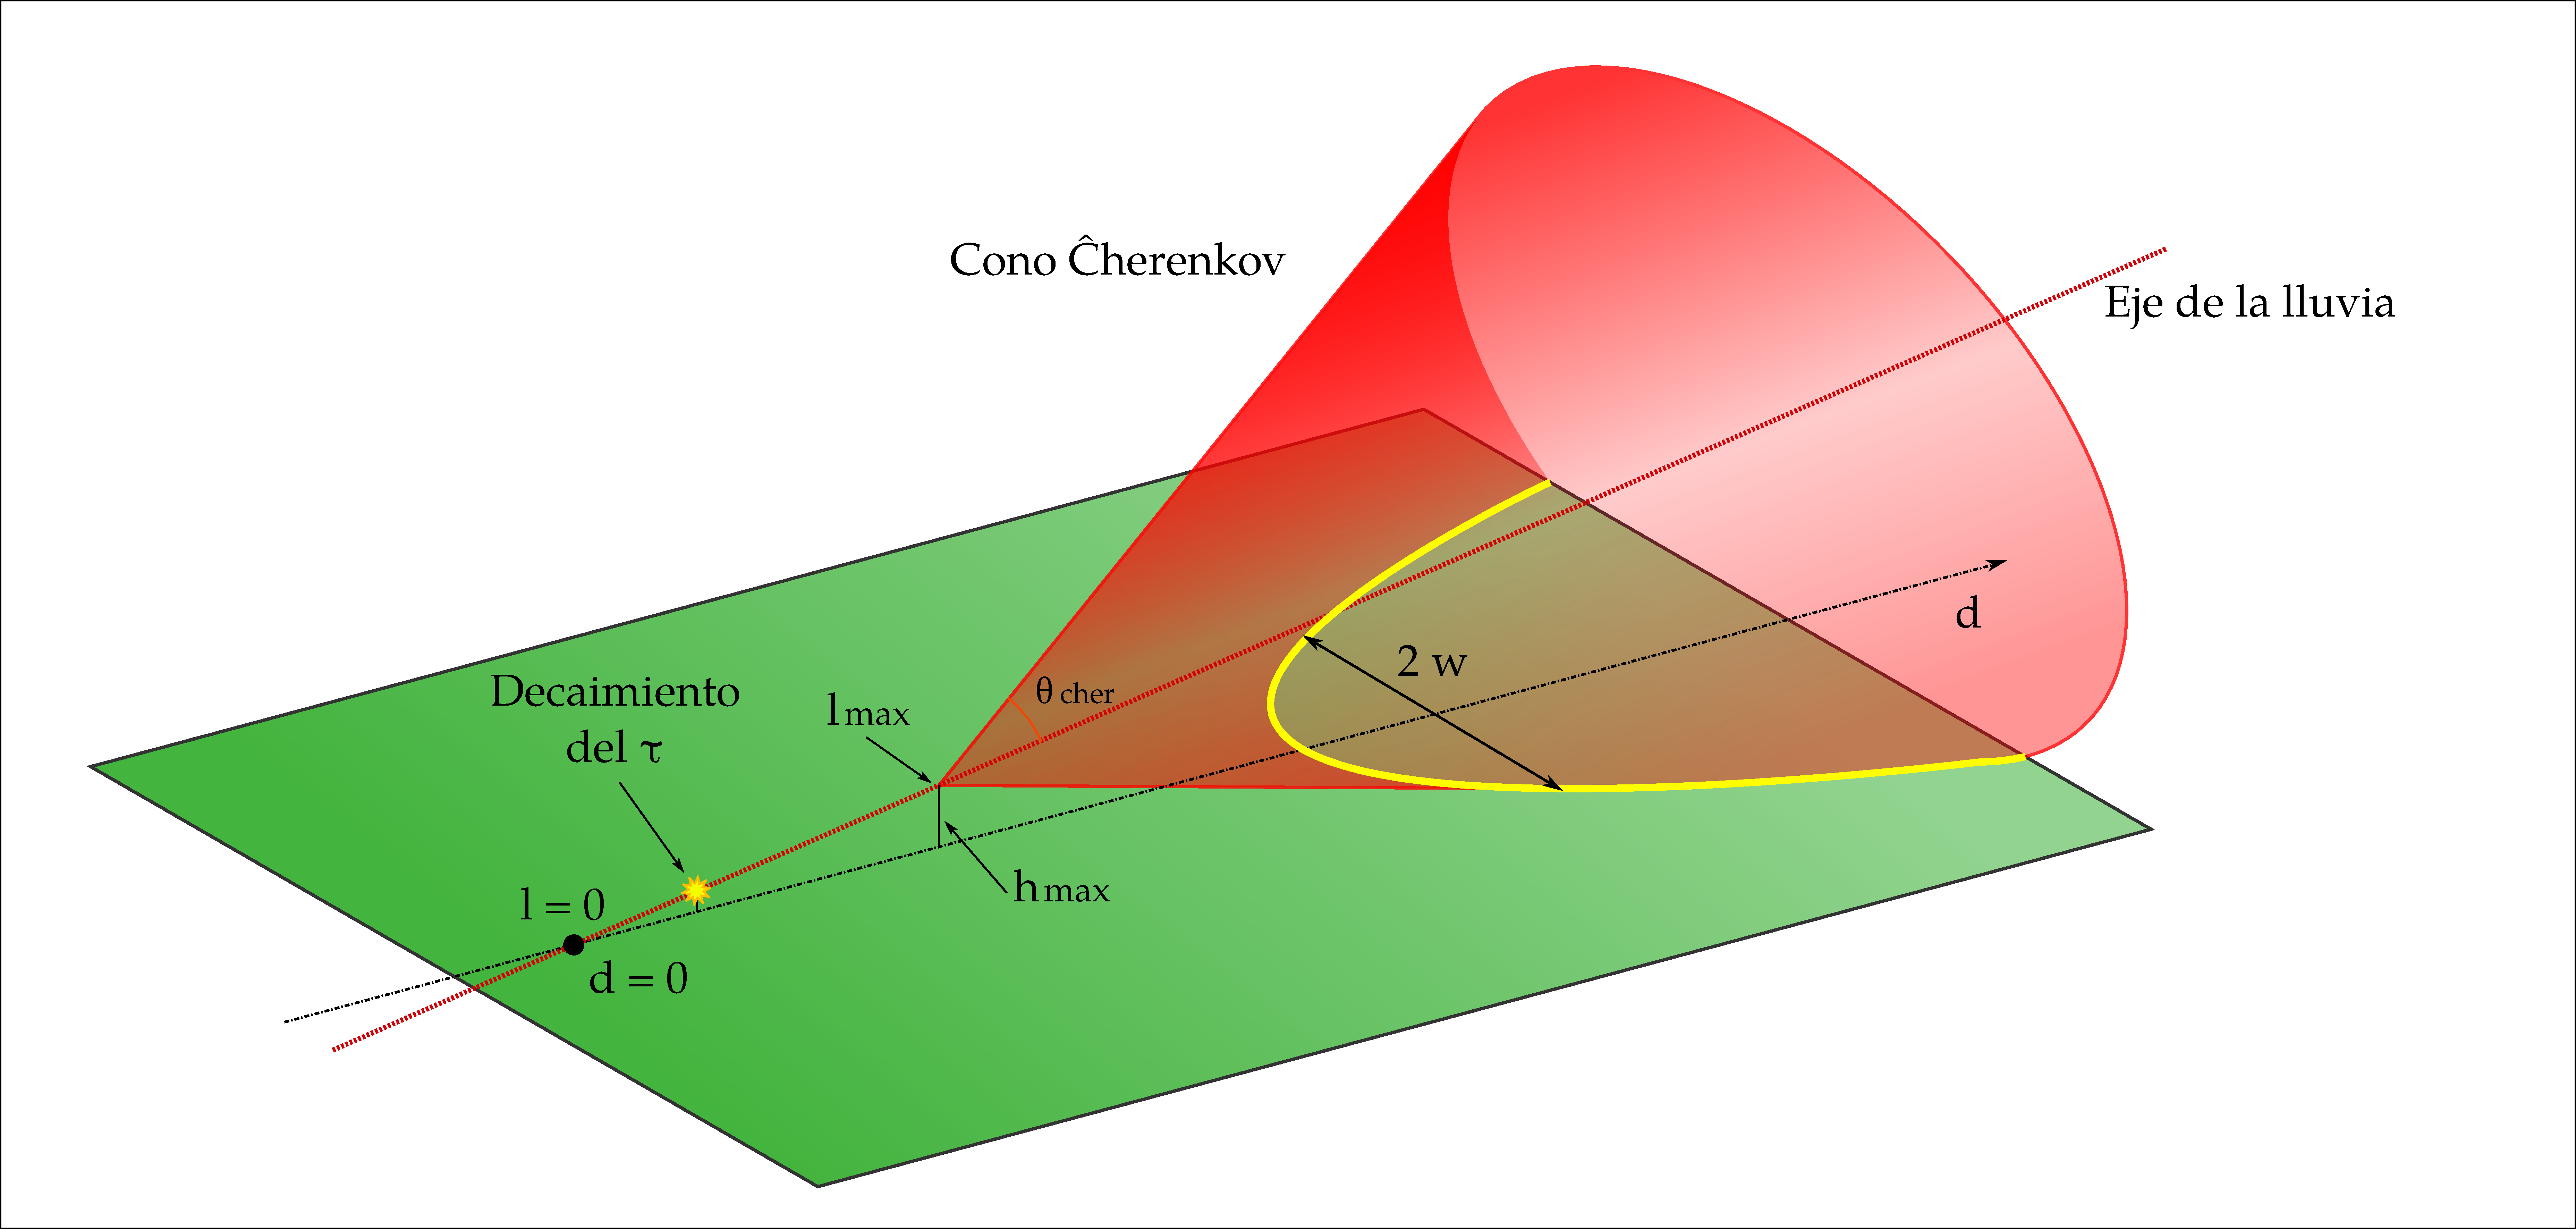
\includegraphics[width=\textwidth]{fig/EASRadio/coneProy}
		\caption{\label{fig:chConeES} La proyección del cono en el suelo para una lluvia ES es ua hip\'erbola.}
	\end{figure}
	%
	Esta hip\'erbola puede ser descripta de manera sencilla, como se muestra en la ecuación \ref{eq:conewidth}, que muestra la expresión con la que se calcula su ancho $w$ como función de la coordenada $d$.
	%
	\begin{equation}
	\renewcommand{\arraystretch}{2.5}
	\begin{array}{rcl}
	w^2&=& \left[\tan^2 \theta_{cher}-\tan^2 \left(\theta-\dfrac{\pi}{2}\right)\right]
	\left(\dfrac{d}{\sin \theta}-l_{max}\right)^2\\
	& & - \tan \left(\theta-\dfrac{\pi}{2}\right) \dfrac{h_{max}}{\sin \theta}
	\left(\dfrac{d}{\sin \theta}-l_{max}\right)
	- \dfrac{h_{max}^2}{\sin^2 \theta}
	\end{array}
	\label{eq:conewidth}
	\end{equation}
	%
	Entran como parámetros el ángulo \cher{} $\theta_{cher}$, el ángulo cenital de la lluvia $\theta$ y la posición del máximo de la lluvia $h_{max}$ y $l_{max}$.
	Los detalles de este cálculo pueden encontrarse en el apendice \ref{ap:intPlanCon}.
	
	La figura \ref{fig:chConeWidth} muestra el ancho en función de $d$ y $\theta$ para \cant{l_{max}=10000}{m} y \cant{h_{max}=l_{max}\cos \theta}{m}.
	\begin{figure}[ht!]
	\centering
		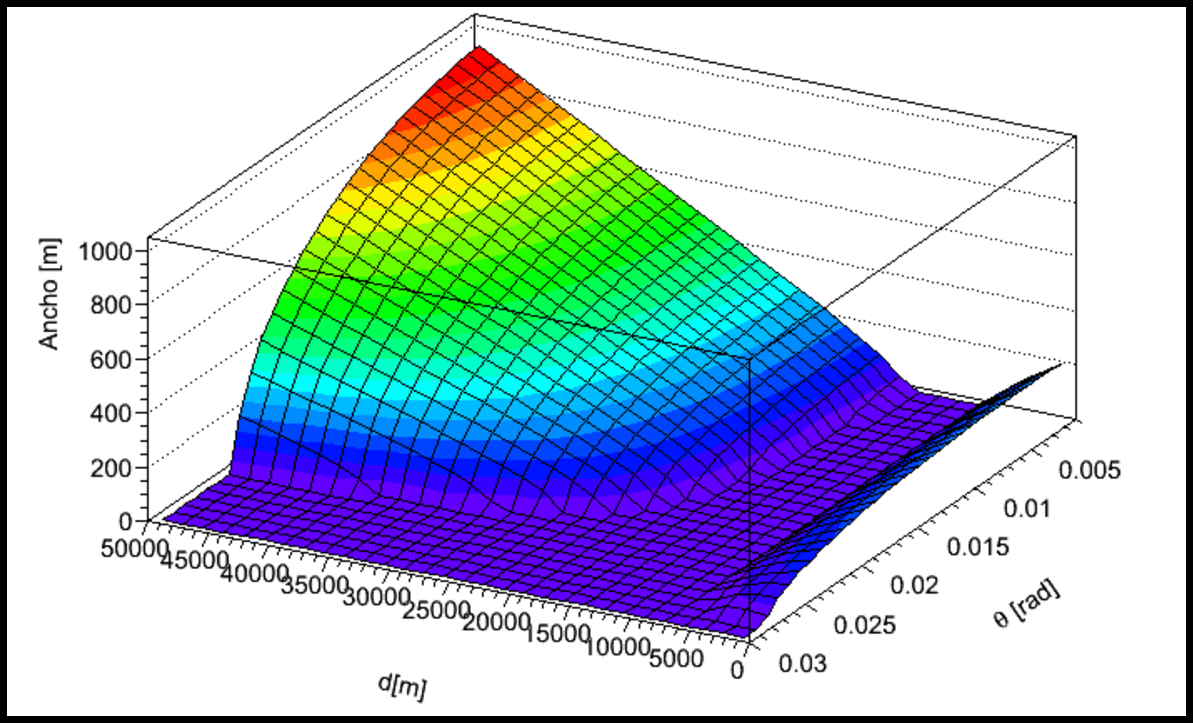
\includegraphics[width=0.85\textwidth]{fig/EASRadio/anchoLluvia}
		\caption{\label{fig:chConeWidth} Ancho $w$ del cono \cher{} como función de $d$ y $\theta$ para \cant{l_{max}=10000}{m} y \cant{h_{max}=l_{max}\cos \theta}{m} (ver geometr\'ia en figura \ref{fig:chConeES}). Los valores del ancho por debajo de \cant{d=10000}{m} corresponden a una solución espúrea de la ecuación \ref{eq:conewidth}.}
	\end{figure}
	La primer observación a esta figura es que la emisión es escencialmente hacia adelante\footnote{De acuerdo con lo expuesto en \ref{sbsc:cher_emision}.}, ya que el ancho es inferior a \cant{1000}{m} para un valor de $d$ en el orden de varios $\rm km$.
	Este aspecto será fundamental a la hora de separar este tipo de lluvias del fondo de lluvias iniciadas por protones o núcleos alto en la atmósfera.
	La segunda observación es que existe un ángulo de corte $\theta_{cut}=90^\circ+\theta_{cher}$ a partir del cuál el cono \cher{} con v\'ertice en el m\'aximo de la lluvia calculado teóricamente no impacta contra el suelo (la ecuación \ref{eq:conewidth} no tiene solución real si el término $\tan^2 \theta_{cher}-\tan^2 (\theta-\frac{\pi}{2})$ es negativo).
	De aquí se desprende que el máximo ángulo cenital con el que un detector de superficie de radio podría ser disparado será del orden de $92^\circ$, es decir, $2^\circ$ por debajo de la l\'inea del horizonte.
	%algunos grados menos que el detector de supeficie del Observatorio Pierre Auger ($\sim95^\circ$).
	
	\subsection{Modelo simplificado para eventos ES}
	\label{sc:toymodelES}

	Adem\'as del cambio en la posici\'on de los m\'aximos de se\~nal dados por la zona de impacto del cono \cher{}, es posible mediante argumentos simples basados en lo expuesto en las secciones previas, recuperar varias caracter\'isticas importantes de la se\~nal de eventos ES a nivel del suelo.
	Para ello, se sigue la filosofía utilizada en~\cite{zhairezAir}, en el que se desarrolla un modelo simplificado para cascadas verticales.
	
	Se considera que de la tierra emerge un $\tau$ con ángulo cenital $\theta$ y decae a una altura $h_d$, como se esquematiza en la figura \ref{fig:esRadio_schema}. 
	\begin{figure}[ht!]
		\centering
		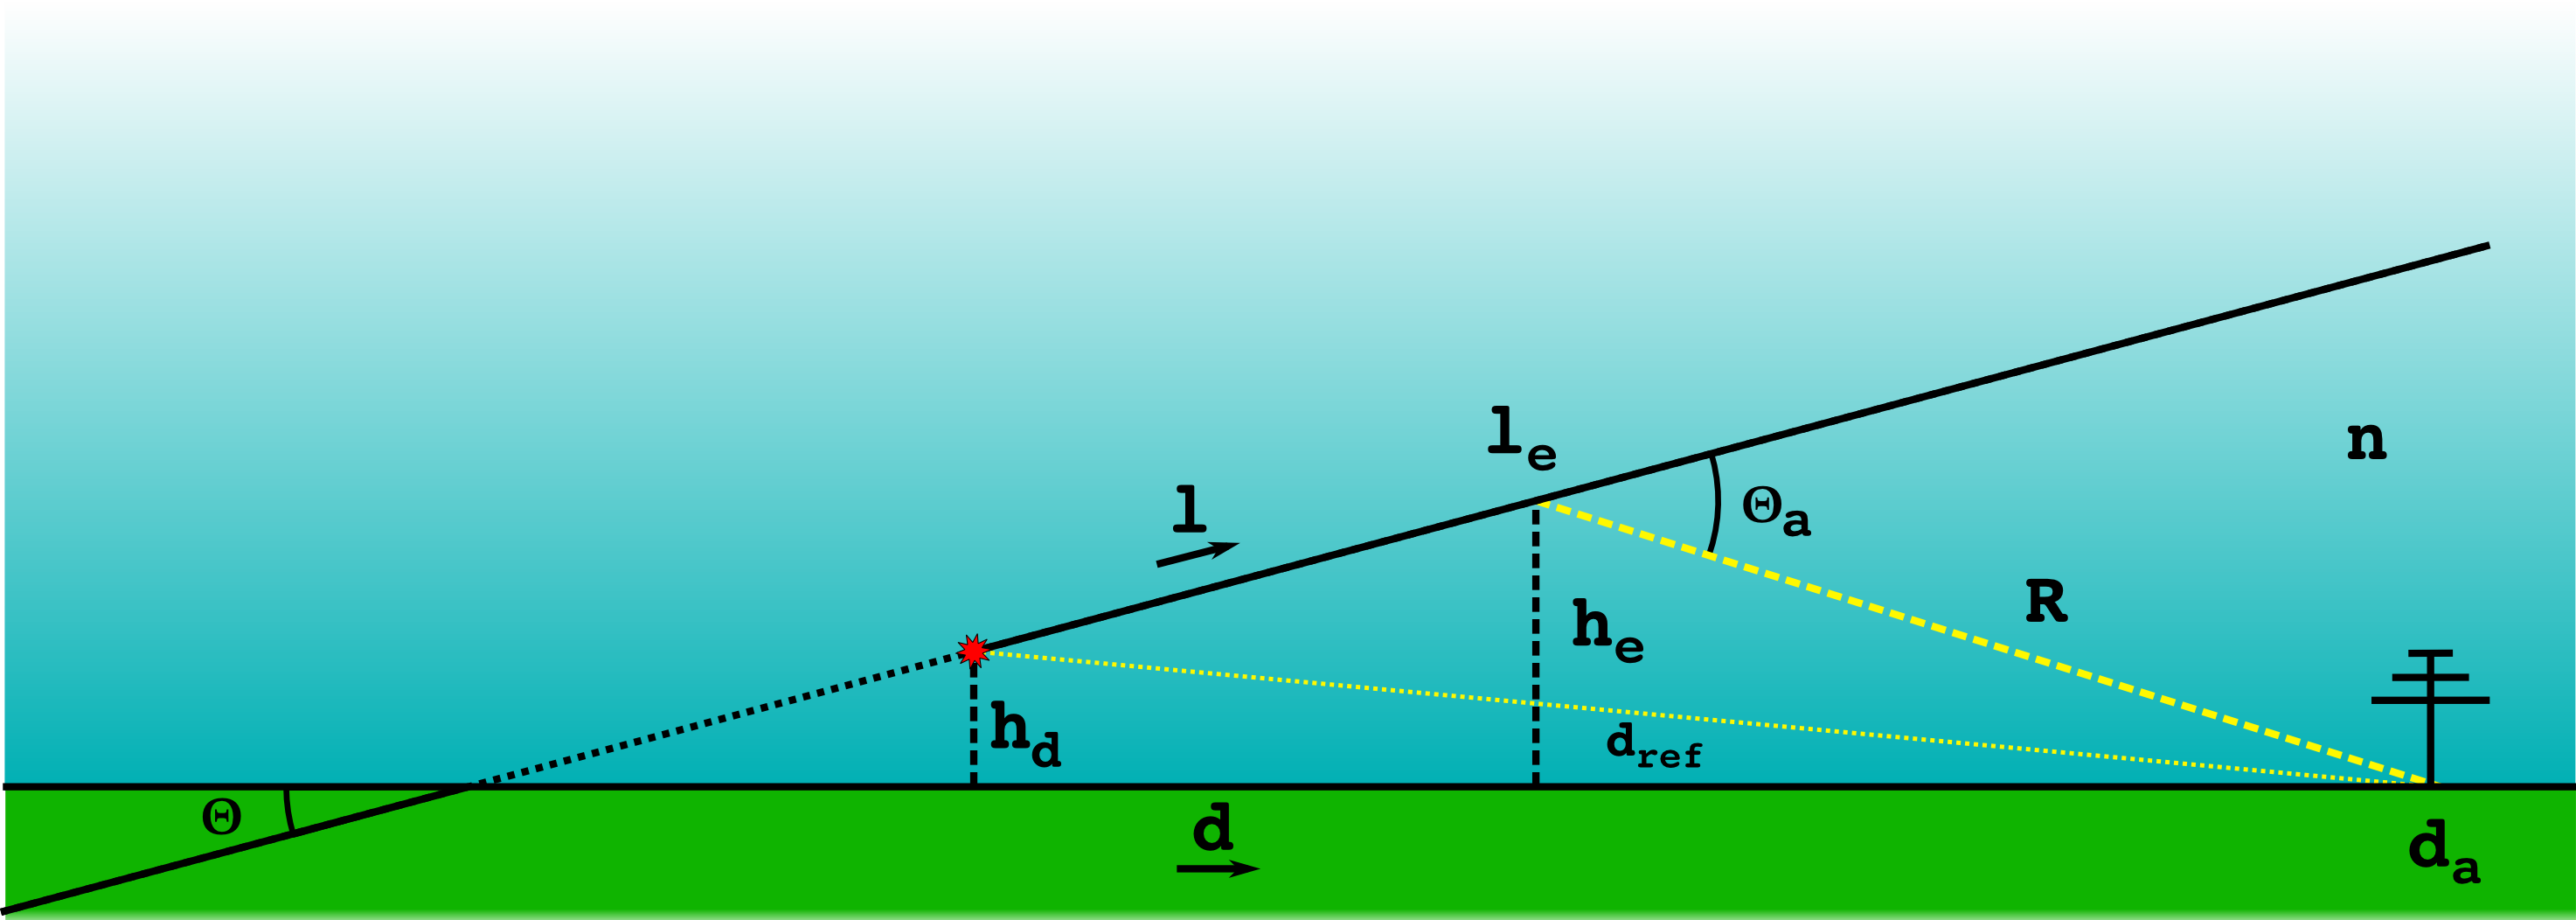
\includegraphics[width=0.95\textwidth]{./fig/EASRadio/timeDelaySchema}
		\caption{\label{fig:esRadio_schema}
		Definici\'on de las variables utilizadas en el modelo simplificado. 
		}
	\end{figure}
	En esta se señalan las coordenadas $d$ y $l$ correspondientes a la distancia sobre el suelo y el eje de la lluvia respectivamente, medidas desde el punto de decaimiento.
	
	El objetivo a partir de aqu\'i es calcular la señal en una antena ubicada en una posición $d_a$ arbitraria.
	Para ello se considerar\'a la señal proveniente de cada punto de emisión $l_e$ de la lluvia, la distancia $R$ entre el punto de emisión y la antena, y la distancia de referencia $d_{ref}$ correspondiente a la que tendr\'ia que recorrer una señal emitida desde el punto de decaimiento.
	Con todo esto, las hipótesis del modelo son las siguientes:
	\begin{enumerate}
	 \item La emisi\'on proviene de una fuente puntual que se desplaza a la velocidad de la luz por el eje de la lluvia.
	 \item El tiempo de llegada de la señal emitida desde $l_e$ a la antena se calcula como la suma del tiempo de llegada del frente hasta $l_e$, partiendo del pundo de decaimiento del $\tau$, m\'as el tiempo que le toma recorrer al pulso desde $l_e$ hasta la antena.
	 \item Si las señales correspondientes a dos puntos de emisión llegan al mismo tiempo\footnote{Se considera que llegan al mismo tiempo si coinciden dentro del mismo bin temporal de \cant{1}{ns}.} a la antena, se suman.
	 \item La señal emitida desde $l_e$ tiene un peso correspondiente al producto entre una Gaiser-Hillas en ese punto (proporcional al n\'umero de part\'iculas de la lluvia) y el factor $1/R$ ($R$ es la distancia entre el punto de emisión y la antena).
	\end{enumerate}
	
	Utilizando 1 y 2, el retardo de la señal como función del ángulo $\theta$ de la lluvia, de la altura de decaimiento $h_d$ del $\tau$, de la posición del observador $d_a$ y del punto de emisión es:
	%
	\begin{equation}
	\begin{array}{rcl}
	t & = & \frac{1}{c}\left[l_e+nR(d_a,l_e,h_d,\theta)-n\,d_{ref}(d_a,l_e,h_d,\theta)\right]
	\end{array}
	\label{eq:toytimedelay1}
	\end{equation}
	%
	donde pueden distinguirse las tres contribuciones expuestas en el punto 2, el tiempo que tarda el frente en llegar a $l_e$, el tiempo que le toma a la señal llegar desde el punto de emisión a la antena a través de un medio de índice de refracción $n$ y se resta el tiempo de referencia que necesita para recorrer $d_{ref}$.
	Luego, utilizando trigonometría básica sobre lo definido en la figura \ref{fig:esRadio_schema} se consigue:
	%
	\begin{equation}
	\begin{array}{rcl}
	t & =  & 
	 \dfrac{1}{c}\left[l_e +
		n \sqrt{h_d^2+d_a^2+l_e^2+2h_dl_e \sin\theta - 2d_al_e\cos\theta} 
		-
		n \sqrt{h_d^2+d_a^2}
		\right]
	\end{array}
	\label{eq:toytimedelay2}
	\end{equation}
	
	A partir de aquí, se fijan dos de los cuatro parámetros: $\theta=90.5^\circ$ y \cant{h_d=50}{m}, valores t\'ipicos en los que se espera tener sensibilidad a \nutau{}'s con radio (ver cap\'itulo \ref{ch:resultadosRadio}).
	En la figura \ref{fig:timeDelay_at} se grafica $t(l)$ en estas condiciones para diferentes observadores (distintos valores de $d_a$).
	\begin{figure}[ht!]
		\centering
		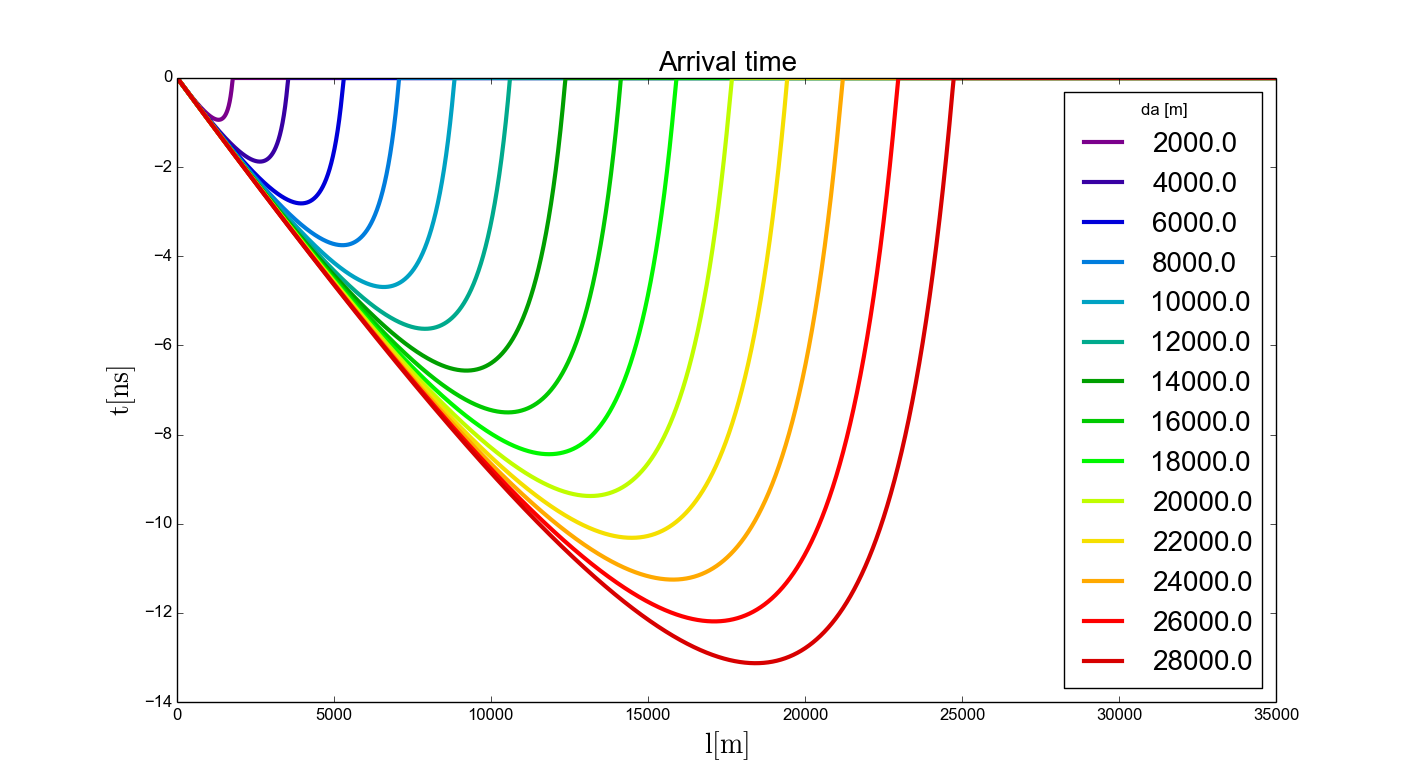
\includegraphics[width=\textwidth]{./fig/EASRadio/timeDelay_at}
		\caption{\label{fig:timeDelay_at}
		Tiempo de arrivo respecto de $d_{ref}/c$ como funci\'on del punto de emisi\'on $l$ a lo largo del eje de la lluvia. Los distintos colores representan antenas a diferentes distancias $d_a$ del punto de $l=0$, que corresponde al punto de decaimiento del \tauon{}, es decir, la posici\'on en la que se inicia la lluvia atmosf\'erica extendida.
		}
	\end{figure}
	Para una cierta posición de la antena $d_a$, el tiempo de arrivo de la se\~nal que proviene de $l=0$ se considera el tiempo de referencia (ver ecuaci\'on \ref{eq:toytimedelay1}), por ello todas las curvas comienzan en $t=0$.
	La pendiente negativa al comienzo se debe a que si bien el trayecto que hay que considerar es mayor que la distancia de referencia ($l_e+R>d_{ref}$ en la figura \ref{fig:esRadio_schema}), la primer parte del recorrido lo realiza la lluvia a velocidad $c$ y la segunda la señal a $c/n$,  por consiguiente, el tiempo de arrivo obtenido es negativo ($t<0$).
	En otras palabras, una se\~nal emitida m\'as tarde desde la lluvia puede llegar antes al detector que una emitida m\'as temprano, como se discuti\'o en la secci\'on \ref{sbsc:cher_emision}.
	Este efecto llega a un máximo para cierto valor de $l$, generando un tiempo de arrivo mínimo, y luego disminuye para valores de $l$ grandes, como muestra la curva de pendiente positiva.
	Como indica el punto 3 del modelo, si la señal proveniente de dos lugares de la lluvia llegan a cierta antena \emph{al mismo tiempo} estas se suman, por lo que los bines temporales con mayor señal serán tales que $dt/dl\sim0$. Este fen\'omeno se denomina compresi\'on temporal.
	
	Por otro lado, tambien será necesario considerar el peso asignado por el modelo al punto $l_e$, como se indica en el punto 4. 
	Dado que por hip\'otesis la emisi\'on total que proviene de un dado punto es proporcional a la densidad de partículas en el mismo, es razonable pesar utilizando una función de Gaiser-Hillas.
	Por otro lado, hay que tener en cuenta el decaimiento del término de radiación que va como $1/R$ (ecuaci\'on \ref{eq:efield_0}).
	En la figura \ref{fig:timeDelay_pd} se muestra en línea punteada la distribución de Gaiser-Hillas para una lluvia cuyo máximo se encuentra a los \cant{10000}{m} del inicio (\cant{\sim10^{18}}{eV}), mientras que en línea llena se grafica el término $1/R$ para diferentes valores de $d_a$.
	\begin{figure}[ht!]
		\centering
		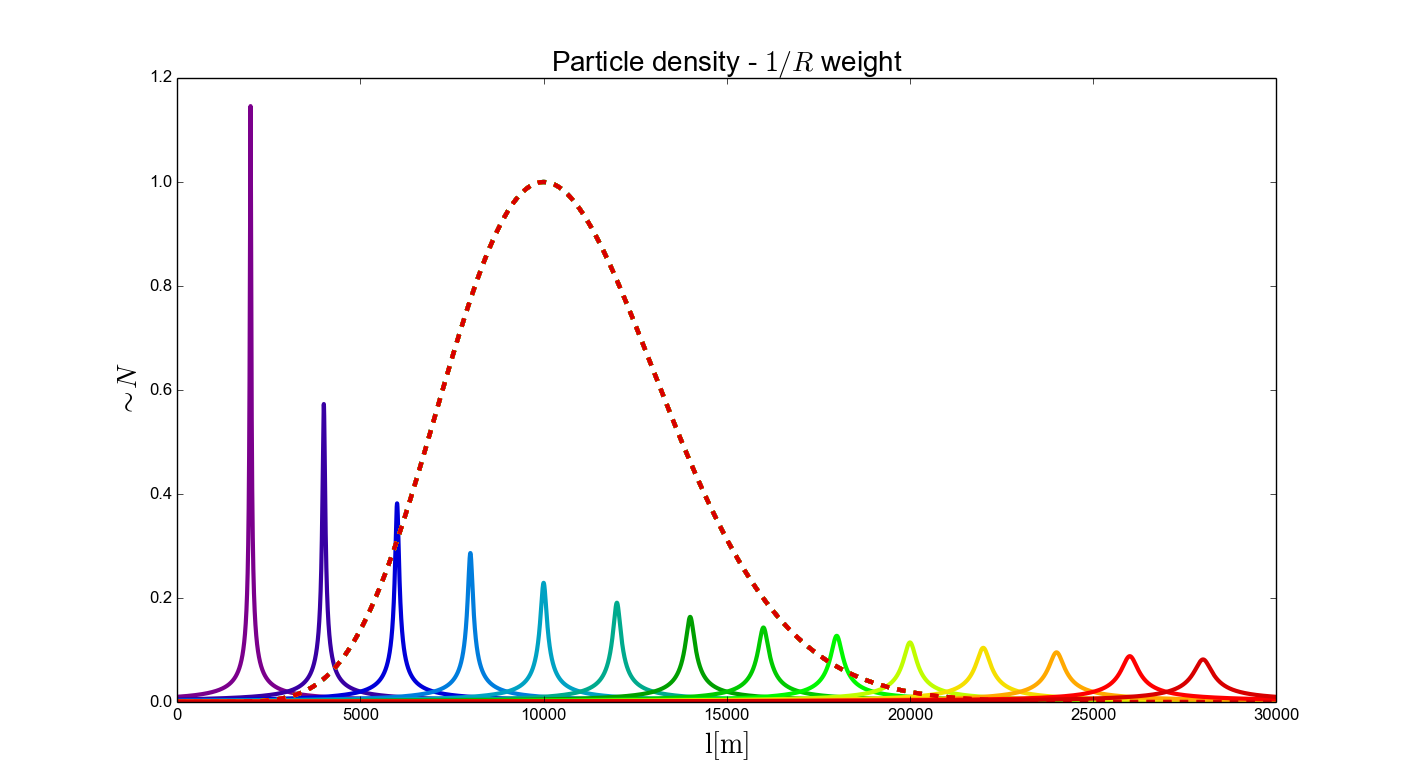
\includegraphics[width=\textwidth]{./fig/EASRadio/timeDelay_pd}
		\caption{\label{fig:timeDelay_pd}
		En l\'inea punteada se muestra la distribuci\'on de part\'iculas a lo largo del eje de la lluvia (coordenada $l$). En l\'inea llena se grafica el factor $1/R$ para antenas en diferentes posiciones $d_a$ seg\'un el c\'odigo de colores de la figura \ref{fig:timeDelay_at}.
		El campo el\'ectrico registrado en cada antena ser\'a proporcional al producto de estas dos funciones.
		}
	\end{figure}
	A la hora de sumar las señales en cada bin temporal se utilizará el producto de ambas curvas para cada antena.
	
	Con los pesos calculados es posible integrar sobre la variable $t$ las curvas de la figura \ref{fig:timeDelay_at}:
	%
	\begin{equation}
	S(t_i)=\sum_{l_i}w_i\Delta l_i
	\label{eq:tint}
	\end{equation}
	%
	donde, $S(t_i)$ es la señal recibida en $t_i\leq t<t_{i+1}$, $\Delta l_i$ es la longitud del intervalo definido por $l_i:t_i\leq t(l_i)<t_{i+1}$ y $w_i=N_i/R_i$ es su peso.
	El resultado de esta integral se expone en la figura \ref{fig:timeDelay_as} para diferentes valores de $d_a$.
	%
	\begin{figure}[ht!]
		\centering
		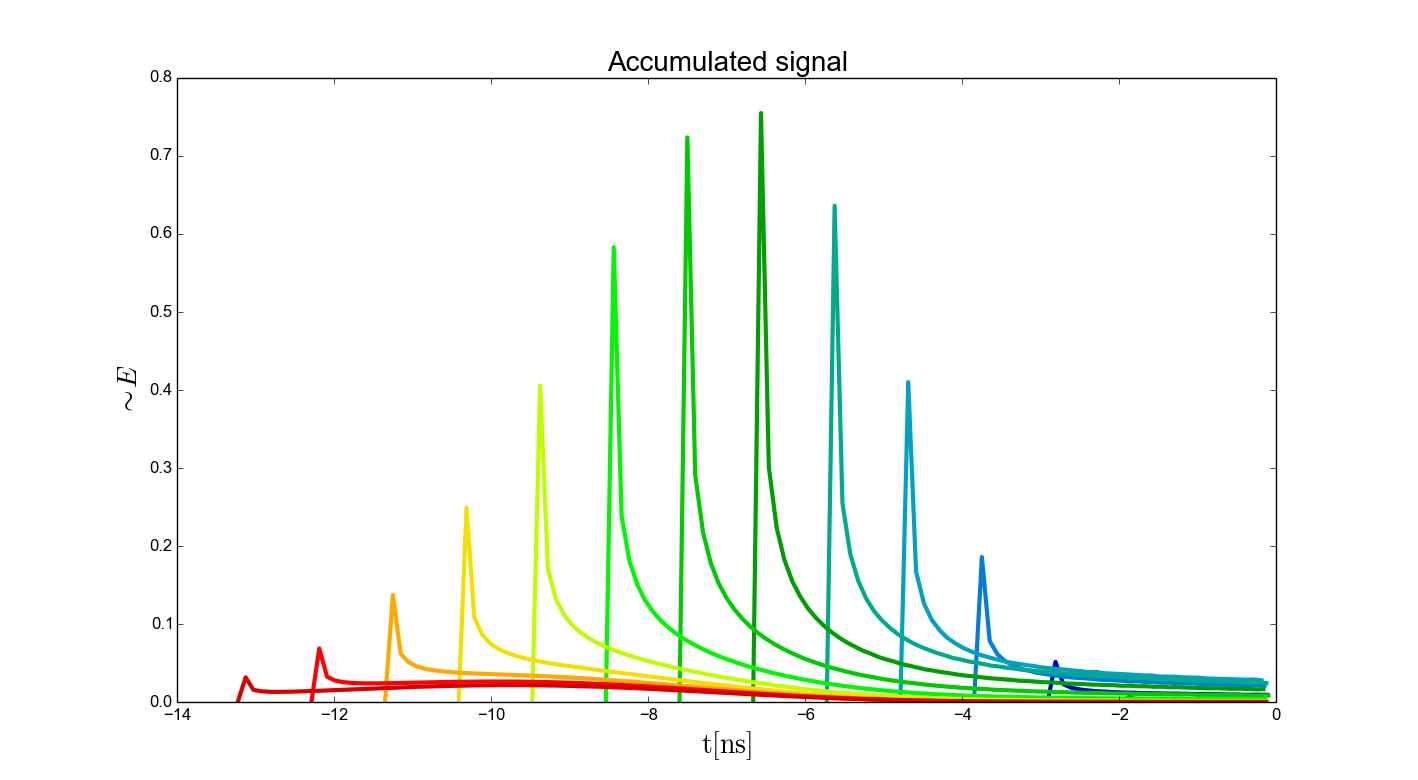
\includegraphics[width=\textwidth]{./fig/EASRadio/timeDelay_as}
		\caption{\label{fig:timeDelay_as}
		Se\~nal acumulada en funci\'on del tiempo, obtenida mediante el modelo aproximado (a partir de la ecuación \ref{eq:tint}) para distintos valores de $d_a$ seg\'un el c\'odigo de colores de la figura \ref{fig:timeDelay_at}.
		}
	\end{figure}
	Cada curva representa la se\~nal en funci\'on del tiempo que registrar\'ia cada antena bajo las suposiciones del modelo, donde se combinan los efectos de la compresi\'on temporal y la combinaci\'on de los pesos correspondientes a la funci\'on de Gaiser-Hillas y a la distancia entre la antena y el eje de la lluvia.
	
	Cabe destacar que el adelanto de la señal respecto de la referencia (frente que se desplaza a velocidad $c$) es del orden de la decena de $\rm ns$, mientras que las antenas se encuentran separadas por alrededor de \cant{2000}{m} entre s\'i, o \cant{6000}{ns} a la velocidad de la luz.
	Por este motivo es razonable suponer que en este tipo de lluvias (ES) la señal a nivel del suelo se desplaza a la velocidad de la luz.
	
	Finalmente, la figura \ref{fig:timeDelay_spa} muestra como es la evolución del máximo de la señal como función de $d_a$.	
	\begin{figure}[ht!]
		\centering
		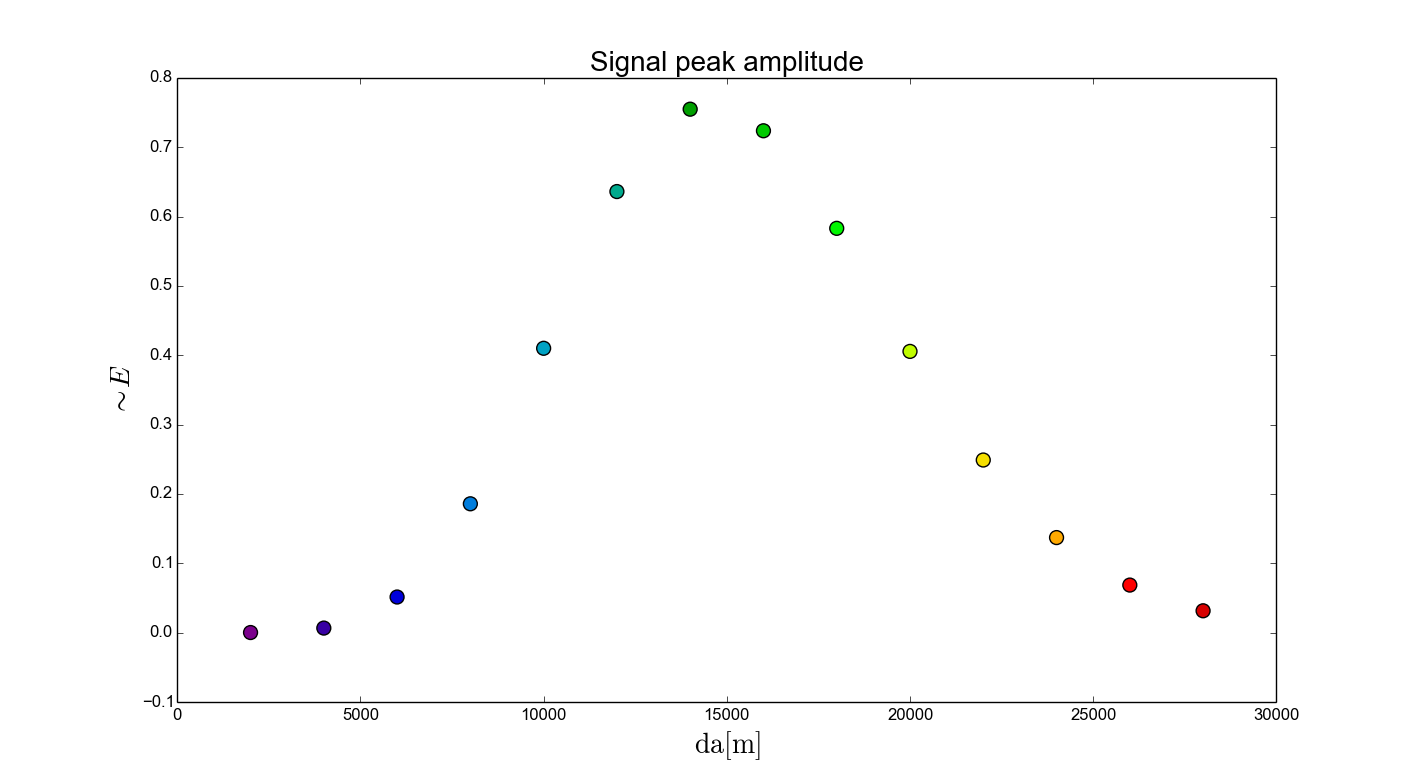
\includegraphics[width=\textwidth]{./fig/EASRadio/timeDelay_spa}
		\caption{\label{fig:timeDelay_spa}
		M\'aximo de la se\~nal acumulada (ver figura \ref{fig:timeDelay_as}) como función de la posici\'on de la antena.
		}
	\end{figure}
	Esta presenta un máximo que se ubica en \cant{\sim 14000}{m}, la posición en la que se espera el máximo según lo expuesto en la sección \ref{sbsc:conoEs} si se considera un cono \cher{} de $1.4^\circ$.
	